\section{W1: Operating Systems}
\textbf{CPU cycle:} fetch, decode, execute, store.\\
\textbf{Registers:} hold variables and temporary results.\\
\textbf{Special registers:} program counter (PC), stack pointer (SP), program status word (PSW).\\
\textbf{User mode:} restricted access to memory and instructions.\\
\textbf{Kernel mode:} full access to the above.\\
\textbf{Memory stack:}\\
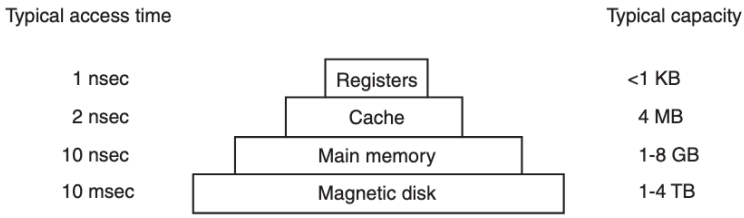
\includegraphics[width=\linewidth]{figs/memory-stack.png}

\subsection{System calls}
\begin{enumerate}
    \item Put system call number in register of OS.
    \item Execute trap instruction (switch to kernel mode).
    \item OS executes system call from fixed address in kernel memory.
    \item The kernel code that starts following the trap instruction is called the \textbf{trap handler}. Trap handler examines the system call number and dispatches the correct system-call handle.
    \item System call handler runs.
    \item Return to user mode.
\end{enumerate}
